\section{Particle Physics}
To be able to understand the scope of the project and the applicability of the work in modern research, this chapter gives an overview of the key concepts from particle physics that appear through the paper. The explanation is written with readers with no prior background in physics in mind.

\subsection{Standard Model}
A non-exhaustive list of the elementary particles is described below, with particles that this report is concerned about (as they appear in the proton-proton collisions) being highlighted.

\begin{itemize}[leftmargin=7mm]
  \item Fermions
  \begin{itemize}[leftmargin=5mm]
    \item Leptons - participate in electroweak interactions; include electron (e\textsuperscript{-})
    \item Quarks - participate in strong interactions; include \textbf{light quarks (q)}\footnote{Light flavor quarks: up (u), down (d), charm (c), and strange (s) quarks} and \textbf{top (t) quark}
  \end{itemize}
  \item Bosons
  \begin{itemize}[leftmargin=5mm]
    \item Gauge bosons - force carriers; include photon ($\gamma$), \textbf{W boson (W\textsuperscript{+}, W\textsuperscript{-})}, \textbf{Z boson}, \textbf{gluons}
    \item Scalar bosons - give rise to mass; include \textbf{Higgs boson (H\textsuperscript{0})}
  \end{itemize}
\end{itemize}

The information about the following decay processes form the dataset of this report, with visualization in figure \ref{fig:jedi-jets} (obtained from \cite{9-newman2019jedi-net:}). It is important to note, that where applicable, the particles on the left-hand side of the arrows undergo a series of decays before reaching the right-hand side, when the only particles left are those composed of quarks and antiquarks (denoted by the vertical bar), referred to as hadrons.

\[ q / g \]
\[ H^0 / W / Z \rightarrow q\overline{q} \]
\[ t \rightarrow Wq \rightarrow q\overline{q}q \]

\begin{figure}[hpt!]
  \centering
  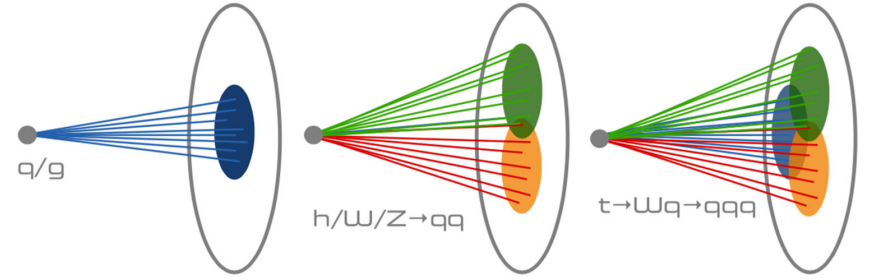
\includegraphics[trim={0cm 0cm 0cm 0cm}, width=0.6\textwidth, center]{background/jedi_jets.png}
  \caption{Representation of different decay processes, based on the number of resulting jet clusters}
  \label{fig:jedi-jets}
\end{figure}

\subsection{Particle Accelerators and triggers at LHC}
The two LHC experiments that are of most concern in this paper are CMS and ATLAS. They are both large general-purpose particle detectors, that were notably involved in the discovery of the Higgs boson \cite{47-greeene2013higgs}. For real-time processing, the detectors are composed of triggers split into levels \citep[p.16]{48-trigger}:

\begin{itemize}
  \item \textbf{Level 1 trigger (L1T)} - it is implemented in hardware (FPGAs) and firmware, pipelined (a term explained in details in \autoref{serial-parallel-pipelined}) and it cannot allow for any dead-time, i.e. has to continuously process data with a fixed latency.
  \item \textbf{Level 2 trigger (L2T)} - it is implemented in hardware and software and can include regional processing.
  \item \textbf{Level 3 trigger (L3T)} - it is implemented in software, using farms of CPUs. It is close in behavior to non-real-time algorithms.
\end{itemize}

Since their origin, the L2T and L3T have been merged into High Level Trigger (HLT) \citep[p.47]{49-tappertriggering}, which is planned to rely on thousands of multithreaded CPUs and GPUs. As for the L1T key specifications that will be used to evaluate the design in this paper, its input data frequency is 40 MHz, which with a pipeline depth of 500 results in a 12.5 \(\mu s\) latency, and its output frequency to HLT is equal to 750 kHz.